\documentclass[10pt,a4paper,noindentfirst]{article}\usepackage[]{graphicx}\usepackage[]{color}
%% maxwidth is the original width if it is less than linewidth
%% otherwise use linewidth (to make sure the graphics do not exceed the margin)
\makeatletter
\def\maxwidth{ %
  \ifdim\Gin@nat@width>\linewidth
    \linewidth
  \else
    \Gin@nat@width
  \fi
}
\makeatother

\definecolor{fgcolor}{rgb}{0.345, 0.345, 0.345}
\newcommand{\hlnum}[1]{\textcolor[rgb]{0.686,0.059,0.569}{#1}}%
\newcommand{\hlstr}[1]{\textcolor[rgb]{0.192,0.494,0.8}{#1}}%
\newcommand{\hlcom}[1]{\textcolor[rgb]{0.678,0.584,0.686}{\textit{#1}}}%
\newcommand{\hlopt}[1]{\textcolor[rgb]{0,0,0}{#1}}%
\newcommand{\hlstd}[1]{\textcolor[rgb]{0.345,0.345,0.345}{#1}}%
\newcommand{\hlkwa}[1]{\textcolor[rgb]{0.161,0.373,0.58}{\textbf{#1}}}%
\newcommand{\hlkwb}[1]{\textcolor[rgb]{0.69,0.353,0.396}{#1}}%
\newcommand{\hlkwc}[1]{\textcolor[rgb]{0.333,0.667,0.333}{#1}}%
\newcommand{\hlkwd}[1]{\textcolor[rgb]{0.737,0.353,0.396}{\textbf{#1}}}%

\usepackage{framed}
\makeatletter
\newenvironment{kframe}{%
 \def\at@end@of@kframe{}%
 \ifinner\ifhmode%
  \def\at@end@of@kframe{\end{minipage}}%
  \begin{minipage}{\columnwidth}%
 \fi\fi%
 \def\FrameCommand##1{\hskip\@totalleftmargin \hskip-\fboxsep
 \colorbox{shadecolor}{##1}\hskip-\fboxsep
     % There is no \\@totalrightmargin, so:
     \hskip-\linewidth \hskip-\@totalleftmargin \hskip\columnwidth}%
 \MakeFramed {\advance\hsize-\width
   \@totalleftmargin\z@ \linewidth\hsize
   \@setminipage}}%
 {\par\unskip\endMakeFramed%
 \at@end@of@kframe}
\makeatother

\definecolor{shadecolor}{rgb}{.97, .97, .97}
\definecolor{messagecolor}{rgb}{0, 0, 0}
\definecolor{warningcolor}{rgb}{1, 0, 1}
\definecolor{errorcolor}{rgb}{1, 0, 0}
\newenvironment{knitrout}{}{} % an empty environment to be redefined in TeX

\usepackage{alltt}

\usepackage[T1]{fontenc}
\usepackage[polish]{babel}
\usepackage[cp1250]{inputenc}
\usepackage{amsmath}
\usepackage{amsfonts}
\usepackage{graphicx}
\usepackage{setspace}
\usepackage{savesym}
\savesymbol{arc}
\usepackage{color}
\usepackage{xcolor}
\usepackage{pict2e}
\usepackage{epstopdf}
\usepackage{geometry}

\newgeometry{tmargin=0.9cm, bmargin=0.9cm, lmargin=0.9cm, rmargin=0.9cm}
\pagestyle{empty}
\linespread{1.2}
\IfFileExists{upquote.sty}{\usepackage{upquote}}{}
\begin{document}

\begin{knitrout}
\definecolor{shadecolor}{rgb}{0.969, 0.969, 0.969}\color{fgcolor}\begin{kframe}
\begin{alltt}
\hlcom{# 2.1}

\hlcom{# a)}

\hlstd{a} \hlkwb{<-} \hlkwd{read.table}\hlstd{(}\hlstr{"http://gamma.mini.pw.edu.pl/~szymanowskih/lab2/OSHORTS.txt"}\hlstd{)}
\hlkwd{head}\hlstd{(a,}\hlnum{2}\hlstd{)}
\end{alltt}
\begin{verbatim}
##    V1
## 1  78
## 2 -58
\end{verbatim}
\begin{alltt}
\hlkwd{acf}\hlstd{(a)}   \hlcom{# ma(1)}
\end{alltt}
\end{kframe}

{\centering \includegraphics[width=\maxwidth]{figure/unnamed-chunk-11} 

}


\begin{kframe}\begin{alltt}
\hlstd{v} \hlkwb{<-} \hlkwd{as.numeric}\hlstd{(}\hlkwd{as.matrix}\hlstd{(a))}\hlopt{-}\hlkwd{mean}\hlstd{(}\hlkwd{as.matrix}\hlstd{(a))}
\hlkwd{Box.test}\hlstd{(v,}\hlkwc{lag}\hlstd{=}\hlnum{20}\hlstd{,}\hlkwc{type}\hlstd{=}\hlstr{"Ljung"}\hlstd{)}   \hlcom{# czyli to nie jest bialy szum}
\end{alltt}
\begin{verbatim}
## 
## 	Box-Ljung test
## 
## data:  v
## X-squared = 38.18, df = 20, p-value = 0.008424
\end{verbatim}
\begin{alltt}
\hlcom{# b)}

\hlstd{ma1} \hlkwb{<-} \hlkwd{arima}\hlstd{(a,}\hlkwd{c}\hlstd{(}\hlnum{0}\hlstd{,}\hlnum{0}\hlstd{,}\hlnum{1}\hlstd{))}
\hlstd{ma1}\hlopt{$}\hlstd{coef}
\end{alltt}
\begin{verbatim}
##       ma1 intercept 
##   -0.8473   -4.7798
\end{verbatim}
\begin{alltt}
\hlkwd{Box.test}\hlstd{(ma1}\hlopt{$}\hlstd{res,}\hlkwc{lag}\hlstd{=}\hlnum{20}\hlstd{,}\hlkwc{type}\hlstd{=}\hlstr{"Ljung"}\hlstd{)}
\end{alltt}
\begin{verbatim}
## 
## 	Box-Ljung test
## 
## data:  ma1$res
## X-squared = 21.81, df = 20, p-value = 0.3509
\end{verbatim}
\begin{alltt}
\hlcom{# c) -> uzyjemy statystyki walda do tego testu}

\hlstd{ma1}\hlopt{$}\hlstd{var.coef}
\end{alltt}
\begin{verbatim}
##               ma1 intercept
## ma1       0.01453   0.02001
## intercept 0.02001   1.05404
\end{verbatim}
\begin{alltt}
\hlstd{stat} \hlkwb{<-} \hlkwd{as.numeric}\hlstd{(ma1}\hlopt{$}\hlstd{coef[}\hlnum{2}\hlstd{]}\hlopt{/}\hlkwd{sqrt}\hlstd{(ma1}\hlopt{$}\hlstd{var.coef[}\hlnum{2}\hlstd{,}\hlnum{2}\hlstd{]))}
\hlstd{p.val} \hlkwb{<-} \hlkwd{pnorm}\hlstd{(stat)}
\hlstd{p.val}
\end{alltt}
\begin{verbatim}
## [1] 1.614e-06
\end{verbatim}
\begin{alltt}
\hlcom{# odrzucamy hipoteze zerowa -> srednia jest ujemna}

\hlcom{# d)}
\hlcom{# przedzial ufnosci dla thety: theta to wspolczynnik w modelu ma(1)}
\hlcom{# xt = epst + theta*eps(t-1) + mi}

\hlstd{qu} \hlkwb{<-} \hlkwd{qnorm}\hlstd{(}\hlnum{0.975}\hlstd{)}
\hlstd{ma1}\hlopt{$}\hlstd{coef[}\hlnum{1}\hlstd{]}\hlopt{+}\hlkwd{sqrt}\hlstd{(ma1}\hlopt{$}\hlstd{var.coef[}\hlnum{1}\hlstd{,}\hlnum{1}\hlstd{])}\hlopt{*}\hlkwd{c}\hlstd{(}\hlopt{-}\hlstd{qu,qu)}
\end{alltt}
\begin{verbatim}
## [1] -1.0835 -0.6111
\end{verbatim}
\begin{alltt}
\hlcom{# 2.2}

\hlkwd{library}\hlstd{(}\hlstr{"MASS"}\hlstd{)}

\hlcom{# a)}

\hlstd{co} \hlkwb{<-} \hlkwd{dget}\hlstd{(}\hlstr{"http://gamma.mini.pw.edu.pl/~szymanowskih/lab2/co2.dput"}\hlstd{)}
\hlkwd{head}\hlstd{(co)}
\end{alltt}
\begin{verbatim}
## [1] 363.1 364.2 364.9 364.5 364.3 362.1
\end{verbatim}
\begin{alltt}
\hlcom{# b)}

\hlkwd{plot}\hlstd{(co)}  \hlcom{# co widac: sezonowosc i trend}
\end{alltt}
\end{kframe}

{\centering 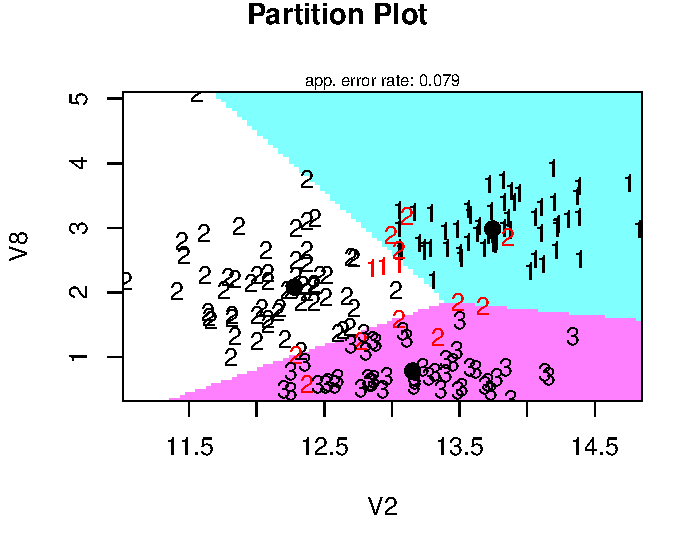
\includegraphics[width=\maxwidth]{figure/unnamed-chunk-12} 

}


\begin{kframe}\begin{alltt}
\hlcom{# c)}

\hlkwd{plot}\hlstd{(}\hlkwd{window}\hlstd{(co,}\hlkwc{start}\hlstd{=}\hlkwd{c}\hlstd{(}\hlnum{2000}\hlstd{,}\hlnum{1}\hlstd{)))}
\hlstd{Month}\hlkwb{=}\hlkwd{c}\hlstd{(}\hlstr{"J"}\hlstd{,} \hlstr{"F"}\hlstd{,}\hlstr{"M"}\hlstd{,}\hlstr{"A"}\hlstd{,}\hlstr{"M"}\hlstd{,}\hlstr{"J"}\hlstd{,}\hlstr{"J"}\hlstd{,}\hlstr{"A"}\hlstd{,}\hlstr{"S"}\hlstd{,}\hlstr{"O"}\hlstd{,}\hlstr{"N"}\hlstd{,}\hlstr{"D"} \hlstd{)}
\hlkwd{points}\hlstd{(}\hlkwd{window}\hlstd{(co,} \hlkwc{start}\hlstd{=}\hlkwd{c}\hlstd{(}\hlnum{2000}\hlstd{,}\hlnum{1}\hlstd{)),} \hlkwc{pch}\hlstd{=Month)}
\end{alltt}
\end{kframe}

{\centering \includegraphics[width=\maxwidth]{figure/unnamed-chunk-13} 

}


\begin{kframe}\begin{alltt}
\hlcom{# d)}

\hlkwd{acf}\hlstd{(co,}\hlkwc{lag.max}\hlstd{=}\hlnum{40}\hlstd{)}   \hlcom{# widac niestacjonarnosc i sezonowosc}
\end{alltt}
\end{kframe}

{\centering \includegraphics[width=\maxwidth]{figure/unnamed-chunk-14} 

}


\begin{kframe}\begin{alltt}
\hlcom{# zeby usunac trend: zroznicujmy}

\hlcom{# e)}

\hlstd{cod} \hlkwb{<-} \hlkwd{diff}\hlstd{(co)}
\hlkwd{plot}\hlstd{(cod)}   \hlcom{# trend usuniety, ale mamy okresowosc}
\end{alltt}
\end{kframe}

{\centering \includegraphics[width=\maxwidth]{figure/unnamed-chunk-15} 

}


\begin{kframe}\begin{alltt}
\hlcom{# f)}

\hlkwd{acf}\hlstd{(cod)}
\end{alltt}
\end{kframe}

{\centering \includegraphics[width=\maxwidth]{figure/unnamed-chunk-16} 

}


\begin{kframe}\begin{alltt}
\hlcom{# g)}

\hlstd{co12} \hlkwb{<-} \hlkwd{diff}\hlstd{(cod,}\hlkwc{lag}\hlstd{=}\hlnum{12}\hlstd{)}
\hlkwd{plot}\hlstd{(co12)}
\end{alltt}
\end{kframe}

{\centering \includegraphics[width=\maxwidth]{figure/unnamed-chunk-17} 

}


\begin{kframe}\begin{alltt}
\hlcom{# lepiej pod tym wzgledem, ze nie widac regularnosci, }
\hlcom{# czyli szereg wyglada na stacjonarny}

\hlcom{# h)}

\hlkwd{acf}\hlstd{(co12)}
\end{alltt}
\end{kframe}

{\centering \includegraphics[width=\maxwidth]{figure/unnamed-chunk-18} 

}


\begin{kframe}\begin{alltt}
\hlcom{# ten rysunek nam mowi, ze pierwsza i dwunasta sa istotne i jeszcze dwie, }
\hlcom{# ale je olewamy :D}

\hlcom{# i)}

\hlcom{# dopasujemy model z pierwszym i dwunastym - model sezonowy}

\hlstd{ma1d} \hlkwb{<-} \hlkwd{arima}\hlstd{(co,}\hlkwc{order}\hlstd{=}\hlkwd{c}\hlstd{(}\hlnum{0}\hlstd{,}\hlnum{1}\hlstd{,}\hlnum{1}\hlstd{),}\hlkwc{seasonal}\hlstd{=}\hlkwd{list}\hlstd{(}\hlkwc{order}\hlstd{=}\hlkwd{c}\hlstd{(}\hlnum{0}\hlstd{,}\hlnum{1}\hlstd{,}\hlnum{1}\hlstd{),}\hlnum{12}\hlstd{))}

\hlcom{# j)}

\hlkwd{plot}\hlstd{(}\hlkwd{residuals}\hlstd{(ma1d))}
\end{alltt}
\end{kframe}

{\centering \includegraphics[width=\maxwidth]{figure/unnamed-chunk-19} 

}


\begin{kframe}\begin{alltt}
\hlcom{# dlaczego pierwsze trzynascie jest podejrzanych? }
\hlcom{# bo dla pierwszych trzynastu brak nam danych - R je sobie przybliza, }
\hlcom{# dlatego sie pojawiaja w ogole}

\hlcom{# k)}

\hlstd{res} \hlkwb{<-} \hlkwd{residuals}\hlstd{(ma1d)[}\hlopt{-}\hlkwd{c}\hlstd{(}\hlnum{1}\hlopt{:}\hlnum{13}\hlstd{)]}
\hlkwd{qqnorm}\hlstd{(res)}
\hlkwd{abline}\hlstd{(}\hlnum{0}\hlstd{,}\hlnum{1}\hlstd{)}
\end{alltt}
\end{kframe}

{\centering \includegraphics[width=\maxwidth]{figure/unnamed-chunk-110} 

}


\begin{kframe}\begin{alltt}
\hlkwd{Box.test}\hlstd{(res,}\hlkwc{type}\hlstd{=}\hlstr{"Ljung"}\hlstd{,}\hlkwc{lag}\hlstd{=}\hlnum{20}\hlstd{)}
\end{alltt}
\begin{verbatim}
## 
## 	Box-Ljung test
## 
## data:  res
## X-squared = 17.94, df = 20, p-value = 0.5915
\end{verbatim}
\begin{alltt}
\hlkwd{shapiro.test}\hlstd{(res)}   \hlcom{# uznajemy, ze rezidua maja rozklad normalny}
\end{alltt}
\begin{verbatim}
## 
## 	Shapiro-Wilk normality test
## 
## data:  res
## W = 0.982, p-value = 0.1134
\end{verbatim}
\begin{alltt}
\hlcom{# l)}

\hlkwd{acf}\hlstd{(res)}
\end{alltt}
\end{kframe}

{\centering \includegraphics[width=\maxwidth]{figure/unnamed-chunk-111} 

}


\begin{kframe}\begin{alltt}
\hlcom{# m)}

\hlstd{pred24} \hlkwb{<-} \hlkwd{predict}\hlstd{(ma1d,}\hlkwc{n.ahead}\hlstd{=}\hlnum{24}\hlstd{)}
\hlkwd{ts.plot}\hlstd{(pred24}\hlopt{$}\hlstd{pred,co,pred24}\hlopt{$}\hlstd{pred}\hlopt{+}\hlnum{2}\hlopt{*}\hlstd{pred24}\hlopt{$}\hlstd{se,}
        \hlstd{pred24}\hlopt{$}\hlstd{pred}\hlopt{-}\hlnum{2}\hlopt{*}\hlstd{pred24}\hlopt{$}\hlstd{se,}\hlkwc{col}\hlstd{=}\hlkwd{c}\hlstd{(}\hlstr{"black"}\hlstd{,}\hlstr{"black"}\hlstd{,}\hlstr{"red"}\hlstd{,}\hlstr{"red"}\hlstd{),}
        \hlkwc{lty}\hlstd{=}\hlkwd{c}\hlstd{(}\hlnum{1}\hlstd{,}\hlnum{1}\hlstd{,}\hlnum{2}\hlstd{,}\hlnum{2}\hlstd{))}
\end{alltt}
\end{kframe}

{\centering \includegraphics[width=\maxwidth]{figure/unnamed-chunk-112} 

}


\begin{kframe}\begin{alltt}
\hlcom{# n)}

\hlstd{pred48} \hlkwb{<-} \hlkwd{predict}\hlstd{(ma1d,}\hlkwc{n.ahead}\hlstd{=}\hlnum{48}\hlstd{)}
\hlkwd{ts.plot}\hlstd{(pred48}\hlopt{$}\hlstd{pred,co,pred48}\hlopt{$}\hlstd{pred}\hlopt{+}\hlnum{2}\hlopt{*}\hlstd{pred48}\hlopt{$}\hlstd{se,}
        \hlstd{pred48}\hlopt{$}\hlstd{pred}\hlopt{-}\hlnum{2}\hlopt{*}\hlstd{pred48}\hlopt{$}\hlstd{se,}\hlkwc{col}\hlstd{=}\hlkwd{c}\hlstd{(}\hlstr{"black"}\hlstd{,}\hlstr{"black"}\hlstd{,}\hlstr{"red"}\hlstd{,}\hlstr{"red"}\hlstd{),}
        \hlkwc{lty}\hlstd{=}\hlkwd{c}\hlstd{(}\hlnum{1}\hlstd{,}\hlnum{1}\hlstd{,}\hlnum{2}\hlstd{,}\hlnum{2}\hlstd{) ,}\hlkwc{xlim}\hlstd{=}\hlkwd{c}\hlstd{(}\hlnum{2004}\hlstd{,}\hlnum{2009}\hlstd{))}
\end{alltt}
\end{kframe}

{\centering \includegraphics[width=\maxwidth]{figure/unnamed-chunk-113} 

}



\end{knitrout}


\end{document}


